\documentclass{article}
\usepackage{graphicx}
\usepackage{fullpage}
\usepackage{mathtools}
\usepackage{amssymb}
\usepackage{listings}
\title{A "quick-and-dirty" implementation of the exponential function}
\author{K. R. ~Pedersen}
\date{}
\begin{document}
\lstset{language=C}
\maketitle

\begin{abstract}
We introduce a simple but "quick-and-dirty" implementation of the exponential function. The implementation will be done in the C-language.
\end{abstract}

\section{Introduction}
The real exponential function $\exp(x)=e^x$ is defined as the limit:

\begin{equation}
e^x = \lim_{n \to \infty} \left(1+\frac{x}{n} \right)^n
\label{def e}
\end{equation}
where $x \in \mathbb{R}$. The function given by Eq. (\ref{def e}) has the remarkable property that it is its own derivative:

\begin{equation}
\frac{\mathrm d}{\mathrm d x} e^x = e^x
	\label{derivative}
\end{equation}

When doing numerical calculations one has to use approximate expressions. In this case it is often useful to consider the Maclaurin series of the exponential function given as

\begin{equation}
e^x=\sum_{n=0}^{\infty} \frac{x^n}{n!}
	\label{series}
\end{equation}

\section{Numerical implementation}
In a numerical implementation of the exponential function, we will always consider only finitely many terms of the series in Eq. (\ref{series}). As an example, note that when including terms up to $n=3$, the series can be written in the form
\begin{equation}
1+x\bigg(1+\frac{x}{2}\bigg(1+\frac{x}{3}\bigg)\bigg),
	\label{rewriting}
\end{equation}
which is naturally extended when including more terms. This rewriting will be the starting point of our "quick-and-dirty" implementation. Written in the C-language, the implementation looks like:
\begin{lstlisting}
double ex(double x){
	if(x<0) return 1/ex(-x);
	if(x>1./8) return pow(ex(x/2),2);
return 1+x*(1+x/2*(1+x/3*(1+x/4*(1+x/5*(1+x/6*(1+x/7*(1+x/8*(1+x/9*(1+x/10)))))))));
}
\end{lstlisting}
On Figure \ref{plot}, a plot of the implementation is presented together with an in-built exponential function implementation. Writing the function in this way has several advantages for numerical calculations. First of all, note that the function always will return a series where each term is positive. This makes the series converge much faster than if the signs of the terms were alternating. Secondly, we make sure that the argument in our function remains small, since when $x>1/8$ we half the argument (and double the value afterwards, such that the total result stays the same). This is to get a better approximation, since the validity of the used Maclaurin polynomial is highest when $x$ is close to $0$. Finally, we make use of the form given in Eq. \ref{rewriting} instead of the more natural form where each term are of the form $\frac{x^n}{n!}$. The reason is that the operation * does not require as much of the program as the more complicated power- and factorial operations. 
\begin{figure}
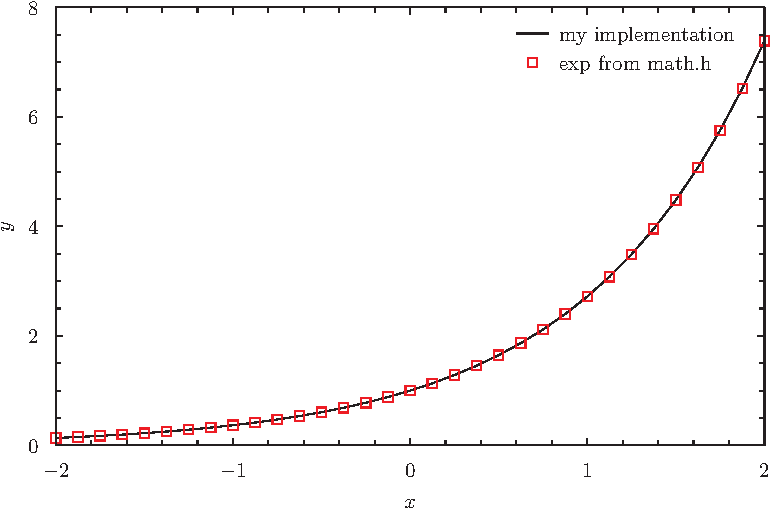
\includegraphics{plot.pdf}
	\caption{A plot of the numerically implementet exponential function}
	\label{plot}
\end{figure}





\end{document} 
